\tikzset{every picture/.style={line width=0.75pt}} %set default line width to 0.75pt        

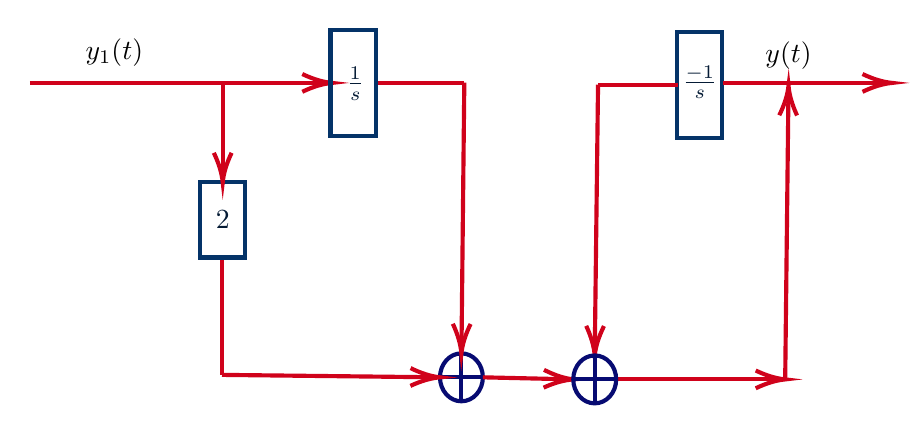
\begin{tikzpicture}[x=0.75pt,y=0.75pt,yscale=-1,xscale=1]
%uncomment if require: \path (0,413); %set diagram left start at 0, and has height of 413

%Straight Lines [id:da5727032991915001] 
\draw [color={rgb, 255:red, 208; green, 2; blue, 27 }  ,draw opacity=1 ][line width=1.5]    (58.56,110.61) -- (161.51,110.61) ;
%Straight Lines [id:da6353712181396247] 
\draw [color={rgb, 255:red, 208; green, 2; blue, 27 }  ,draw opacity=1 ][line width=1.5]    (161.51,110.61) -- (201.08,110.61) ;
\draw [shift={(204.08,110.61)}, rotate = 180] [color={rgb, 255:red, 208; green, 2; blue, 27 }  ,draw opacity=1 ][line width=1.5]    (14.21,-4.28) .. controls (9.04,-1.82) and (4.3,-0.39) .. (0,0) .. controls (4.3,0.39) and (9.04,1.82) .. (14.21,4.28)   ;
%Straight Lines [id:da5829042456704695] 
\draw [color={rgb, 255:red, 208; green, 2; blue, 27 }  ,draw opacity=1 ][line width=1.5]    (341.09,253.46) -- (419.53,253.46) ;
\draw [shift={(422.53,253.46)}, rotate = 180] [color={rgb, 255:red, 208; green, 2; blue, 27 }  ,draw opacity=1 ][line width=1.5]    (14.21,-4.28) .. controls (9.04,-1.82) and (4.3,-0.39) .. (0,0) .. controls (4.3,0.39) and (9.04,1.82) .. (14.21,4.28)   ;
%Shape: Rectangle [id:dp2516520568905628] 
\draw  [color={rgb, 255:red, 4; green, 51; blue, 104 }  ,draw opacity=1 ][line width=1.5]  (370.45,86) -- (392.27,86) -- (392.27,137) -- (370.45,137) -- cycle ;
%Straight Lines [id:da4261405254199824] 
\draw [color={rgb, 255:red, 208; green, 2; blue, 27 }  ,draw opacity=1 ][line width=1.5]    (392.56,110.61) -- (471,110.61) ;
\draw [shift={(474,110.61)}, rotate = 180] [color={rgb, 255:red, 208; green, 2; blue, 27 }  ,draw opacity=1 ][line width=1.5]    (14.21,-4.28) .. controls (9.04,-1.82) and (4.3,-0.39) .. (0,0) .. controls (4.3,0.39) and (9.04,1.82) .. (14.21,4.28)   ;
%Shape: Rectangle [id:dp1355970092994433] 
\draw  [color={rgb, 255:red, 4; green, 51; blue, 104 }  ,draw opacity=1 ][line width=1.5]  (140.62,158.27) -- (162.44,158.27) -- (162.44,194.75) -- (140.62,194.75) -- cycle ;
%Flowchart: Or [id:dp7661436109510428] 
\draw  [color={rgb, 255:red, 7; green, 11; blue, 114 }  ,draw opacity=1 ][line width=1.5]  (256.21,252.46) .. controls (256.21,246.08) and (260.83,240.92) .. (266.53,240.92) .. controls (272.24,240.92) and (276.86,246.08) .. (276.86,252.46) .. controls (276.86,258.83) and (272.24,264) .. (266.53,264) .. controls (260.83,264) and (256.21,258.83) .. (256.21,252.46) -- cycle ; \draw  [color={rgb, 255:red, 7; green, 11; blue, 114 }  ,draw opacity=1 ][line width=1.5]  (256.21,252.46) -- (276.86,252.46) ; \draw  [color={rgb, 255:red, 7; green, 11; blue, 114 }  ,draw opacity=1 ][line width=1.5]  (266.53,240.92) -- (266.53,264) ;
%Straight Lines [id:da4878156257526778] 
\draw [color={rgb, 255:red, 208; green, 2; blue, 27 }  ,draw opacity=1 ][line width=1.5]    (317.43,253.39) -- (276.86,252.46) ;
\draw [shift={(320.43,253.46)}, rotate = 181.31] [color={rgb, 255:red, 208; green, 2; blue, 27 }  ,draw opacity=1 ][line width=1.5]    (14.21,-4.28) .. controls (9.04,-1.82) and (4.3,-0.39) .. (0,0) .. controls (4.3,0.39) and (9.04,1.82) .. (14.21,4.28)   ;
%Straight Lines [id:da01710459462168179] 
\draw [color={rgb, 255:red, 208; green, 2; blue, 27 }  ,draw opacity=1 ][line width=1.5]    (253.21,252.43) -- (151.19,251.28) ;
\draw [shift={(256.21,252.46)}, rotate = 180.64] [color={rgb, 255:red, 208; green, 2; blue, 27 }  ,draw opacity=1 ][line width=1.5]    (14.21,-4.28) .. controls (9.04,-1.82) and (4.3,-0.39) .. (0,0) .. controls (4.3,0.39) and (9.04,1.82) .. (14.21,4.28)   ;
%Straight Lines [id:da46828292830077667] 
\draw [color={rgb, 255:red, 208; green, 2; blue, 27 }  ,draw opacity=1 ][line width=1.5]    (151.19,251.28) -- (151.19,196.16) ;
%Shape: Rectangle [id:dp706545784774389] 
\draw  [color={rgb, 255:red, 4; green, 51; blue, 104 }  ,draw opacity=1 ][line width=1.5]  (203.45,85) -- (225.27,85) -- (225.27,136) -- (203.45,136) -- cycle ;
%Straight Lines [id:da3449564708681504] 
\draw [color={rgb, 255:red, 208; green, 2; blue, 27 }  ,draw opacity=1 ][line width=1.5]    (151.53,155.51) -- (151.53,111.38) ;
\draw [shift={(151.53,158.51)}, rotate = 270] [color={rgb, 255:red, 208; green, 2; blue, 27 }  ,draw opacity=1 ][line width=1.5]    (14.21,-4.28) .. controls (9.04,-1.82) and (4.3,-0.39) .. (0,0) .. controls (4.3,0.39) and (9.04,1.82) .. (14.21,4.28)   ;
%Straight Lines [id:da5817265537026062] 
\draw [color={rgb, 255:red, 208; green, 2; blue, 27 }  ,draw opacity=1 ][line width=1.5]    (226.36,110.5) -- (267.93,110.5) ;
%Straight Lines [id:da11311142092185089] 
\draw [color={rgb, 255:red, 208; green, 2; blue, 27 }  ,draw opacity=1 ][line width=1.5]    (266.57,237.92) -- (267.93,110.5) ;
\draw [shift={(266.53,240.92)}, rotate = 270.61] [color={rgb, 255:red, 208; green, 2; blue, 27 }  ,draw opacity=1 ][line width=1.5]    (14.21,-4.28) .. controls (9.04,-1.82) and (4.3,-0.39) .. (0,0) .. controls (4.3,0.39) and (9.04,1.82) .. (14.21,4.28)   ;
%Straight Lines [id:da794510001898227] 
\draw [color={rgb, 255:red, 208; green, 2; blue, 27 }  ,draw opacity=1 ][line width=1.5]    (370.93,111.5) -- (332.36,111.5) ;
%Straight Lines [id:da7140545147772185] 
\draw [color={rgb, 255:red, 208; green, 2; blue, 27 }  ,draw opacity=1 ][line width=1.5]    (330.8,238.92) -- (332.36,111.5) ;
\draw [shift={(330.76,241.92)}, rotate = 270.7] [color={rgb, 255:red, 208; green, 2; blue, 27 }  ,draw opacity=1 ][line width=1.5]    (14.21,-4.28) .. controls (9.04,-1.82) and (4.3,-0.39) .. (0,0) .. controls (4.3,0.39) and (9.04,1.82) .. (14.21,4.28)   ;
%Flowchart: Or [id:dp9740541329325205] 
\draw  [color={rgb, 255:red, 7; green, 11; blue, 114 }  ,draw opacity=1 ][line width=1.5]  (320.43,253.46) .. controls (320.43,247.08) and (325.05,241.92) .. (330.76,241.92) .. controls (336.46,241.92) and (341.09,247.08) .. (341.09,253.46) .. controls (341.09,259.83) and (336.46,265) .. (330.76,265) .. controls (325.05,265) and (320.43,259.83) .. (320.43,253.46) -- cycle ; \draw  [color={rgb, 255:red, 7; green, 11; blue, 114 }  ,draw opacity=1 ][line width=1.5]  (320.43,253.46) -- (341.09,253.46) ; \draw  [color={rgb, 255:red, 7; green, 11; blue, 114 }  ,draw opacity=1 ][line width=1.5]  (330.76,241.92) -- (330.76,265) ;
%Straight Lines [id:da8593286249198595] 
\draw [color={rgb, 255:red, 208; green, 2; blue, 27 }  ,draw opacity=1 ][line width=1.5]    (424.1,115.04) -- (422.53,253.46) ;
\draw [shift={(424.13,112.04)}, rotate = 90.65] [color={rgb, 255:red, 208; green, 2; blue, 27 }  ,draw opacity=1 ][line width=1.5]    (14.21,-4.28) .. controls (9.04,-1.82) and (4.3,-0.39) .. (0,0) .. controls (4.3,0.39) and (9.04,1.82) .. (14.21,4.28)   ;

% Text Node
\draw (99.28,104.21) node [anchor=south] [inner sep=0.75pt]    {$y_{1}( t)$};
% Text Node
\draw (215.39,110.99) node  [color={rgb, 255:red, 5; green, 27; blue, 53 }  ,opacity=1 ]  {$\frac{1}{s}$};
% Text Node
\draw (381.36,110.24) node  [color={rgb, 255:red, 5; green, 27; blue, 53 }  ,opacity=1 ]  {$\frac{-1}{s}$};
% Text Node
\draw (424.13,105.64) node [anchor=south] [inner sep=0.75pt]    {$y( t)$};
% Text Node
\draw (151.53,176.51) node  [color={rgb, 255:red, 5; green, 27; blue, 53 }  ,opacity=1 ]  {$2$};


\end{tikzpicture}
